

\actTitle{Worksheet 4.1-4.4 Review}

\noindent \textbf{Instructions:}  Work together in groups of  3 or 4 to complete the following problems.\\


\begin{enumerate}

\item Consider the angle $\displaystyle \theta=\frac{7\pi}{4}$ which
  is in standard position.
\begin{enumerate}
\item  Draw a picture labeling $\displaystyle \theta=\frac{7\pi}{4}$
  and it's corresponding reference angle.
  
  \begin{tikzpicture}
    \draw[->,ultra thick] (-5,0)--(5,0) node[right]{$x$};
    \draw[->,ultra thick] (0,-5)--(0,5) node[above]{$y$};
  \end{tikzpicture}

\item Determine the reference angle.
  \vfill

\item Determine $\displaystyle \tan\left(\frac{7\pi}{4}\right)$.
  \vfill
  
\end{enumerate}


\clearpage

%\item Determine the angles, $\theta$, that match the criteria in each question below.
%\begin{enumerate}
%\item An angle that is coterminal with the angle $\alpha=\frac{\pi}{4}$ and is greater than $\pi$.\vfill
%\item An angle that is coterminal with the angle $\alpha=\frac{3\pi}{4}$ and is negative.\vfill
%\end{enumerate}

%\item An angle $\theta$ is in the second quadrant, and $\sin{\theta}=0.25$.  Determine the cosine of the angle.\vfill

\item An angle $\theta$ is in the fourth quadrant, and $\cos{\theta}=0.25$.  Determine the tangent of the angle.\vfill

\item Determine all the angles, $\theta$ between 0 and $3\pi$ such that $\cos{(\theta)}=-\frac{\sqrt{3}}{2}$.  Give exact answers in radians.\vfill




\item The terminal side of an angle $\theta$ in standard position goes
  through the point $(-6,-5).$  Find an exact answer for each of the following.
\begin{enumerate}
\item $\sin{(\theta)}$\vfill
\item $\cos{(\theta)}$\vfill
\item $\cot{(\theta)}$\vfill

\end{enumerate}

\clearpage

\item For each question below, a diagram of a point on a circle is
  given.  Answer each question about the angle formed by the line
  through the point, the origin, and the positive $x$-axis.
\begin{enumerate}
\item Determine the cosine of the angle $\theta$.  (Your answer should
  be a number and not have an $x$ in it.) \\
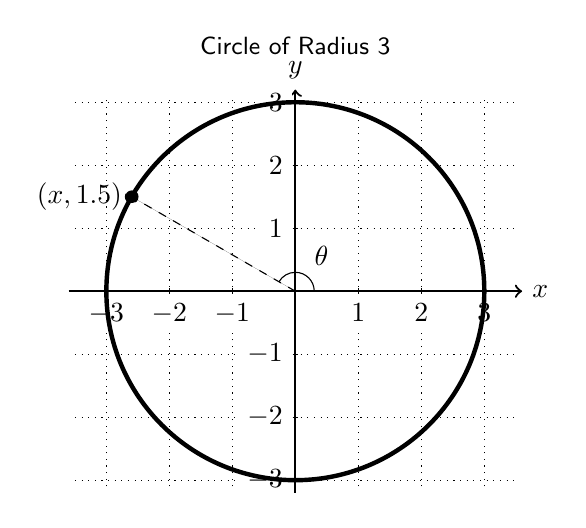
\begin{tikzpicture}[y=0.8cm, x=0.8cm,font=\sffamily]
  \draw[step=1,black, dotted] (-3.5,-3.1) grid (3.5,3.1); % very thin,
  \draw[thick,black,->] (-3.6,0) -- (3.6,0) node[anchor=west] {$x$};
  \draw[thick,black,->] (0,-3.2) -- (0,3.2) node[anchor=south] {$y$};
  \node[black] at (0,3.9) {\small Circle of Radius 3};

  \foreach \x in {-3,-2,-1,1,2,3} {
    \draw (\x,1pt) -- (\x,-1pt);
    \draw (\x,-1pt) node[anchor=north,fill=white] {$\x$};
  }

  \foreach \y in {-3,-2,-1,1,2,3}{
    \draw (-1pt,\y) -- (1pt,\y);
    \draw (-1pt,\y) node[anchor=east,fill=white] {$\y$};
  }

  \draw[ultra thick,black] (0,0) circle(3);
  \draw[black,dashed,fill=black] (0,0) -- (150:3) circle (0.1) node[anchor=east] {$(x,1.5)$};
  \node[black,anchor=south west] at (60:0.3)  {$\theta$};
  \draw[thin,black] (0:0.3) arc (0:150:0.3);
\end{tikzpicture}


\item Determine the tangent of the angle $\psi$.
  (Your answer should be a number and not have a $y$ in it.)\\
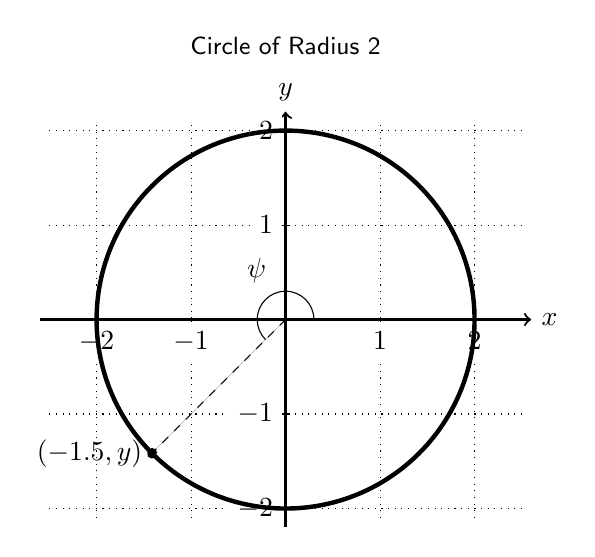
\begin{tikzpicture}[y=1.2cm, x=1.2cm,font=\sffamily]
  \draw[step=1,black, dotted] (-2.5,-2.1) grid (2.5,2.1); % very thin,
  \draw[thick,black,->] (-2.6,0) -- (2.6,0) node[anchor=west] {$x$};
  \draw[thick,black,->] (0,-2.2) -- (0,2.2) node[anchor=south] {$y$};
  \node[black] at (0,2.9) {\small Circle of Radius 2};

  \foreach \x in {-2,-1,1,2} {
    \draw (\x,1pt) -- (\x,-1pt);
    \draw (\x,-1pt) node[anchor=north,fill=white] {$\x$};
  }

  \foreach \y in {-2,-1,1,2}{
    \draw (-1pt,\y) -- (1pt,\y);
    \draw (-1pt,\y) node[anchor=east,fill=white] {$\y$};
  }

  \draw[ultra thick,black] (0,0) circle(2);
  \draw[black,dashed,fill=black] (0,0) -- (225:2) circle (0.05) node[anchor=east] {$(-1.5,y)$};
  \node[black,anchor=south east] at (110:0.3)  {$\psi$};
  \draw[thin,black] (0:0.3) arc (0:225:0.3);
\end{tikzpicture}

\end{enumerate}




\item Given the following, find the exact value of $\sin{(\alpha)}.$\\
  $$\cos{(\alpha)}=-\frac{1}{3} \quad
  \text{and}\quad \tan{(\alpha)} \quad \text{is negative}$$
  Which quadrants could the angle be in?
  \vfill

  \clearpage
  
\item A ship is anchored a distance of $d=150$m from a beach.  A
  spotlight on the bow of the ship can rotate, and the angle is
  measured from a line perpendicular to the beach that goes through
  the base of the spotlight.  Determine the position, $y$, along the
  beach that the spotlight will illuminate the given angle, $\theta$.
  (Your answer should be a function of $\theta$
  with $-\pi/2<\theta <\pi/2.)$\\
  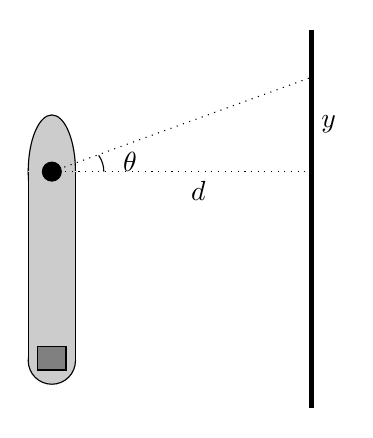
\begin{tikzpicture}[y=1.2cm, x=1.2cm,font=\sffamily]
    %\node[black] at (0,2.9) {\small Circle of Radius 2};

    %\draw[ultra thick,black] (0,0) circle(2);
    %\draw[black,dashed,fill=black] (0,0) -- (225:2) circle (0.05) node[anchor=east] {$(-1.5,y)$};
    %\node[black,anchor=south east] at (110:0.3)  {$\psi$};
    %\draw[thin,black] (0:0.3) arc (0:225:0.3);

    \filldraw[black!20] (0.25,0) circle (0.25);
    \filldraw[black!20] (0.25,2) ellipse (0.25 and 0.6);
    \draw[black] (0.25,2) ellipse (0.25 and 0.6);
    \draw[black] (0.25,0) circle (0.25);
    \filldraw[black!20] (0,0) rectangle(0.5,2);
    \draw[black,fill=black!50] (0.1,-0.1) rectangle(0.4,0.15);
    \draw[black] (0,0) -- (0,2);
    \draw[black] (0.5,0) -- (0.5,2);
    \filldraw[black] (0.25,2) circle(0.1);

    \draw[black,dotted] (0.25,2) -- (3,2);
    \draw[black,dotted] (0.25,2) -- (3,3);
    \draw[black,ultra thick] (3,-0.5) -- (3,3.5);
    \draw[black] (0.8,2) arc (0:35:0.3);

    \node[anchor=west] at (0.9,2.1) {$\theta$};
    \node[anchor=north] at (1.8,2) {$d$};
    \node[anchor=west] at (3,2.5) {$y$};
  \end{tikzpicture}

  

\item A surveyor wishes to determine the height of a building. The
  surveyor is standing directly in front of the building and measures
  an angle of elevation of $17^\circ$ to the top of the building. The
  surveyor then backs up ten meters and measures an angle of
  elevation of $14^\circ$. What is the height of the building?

  \vfill
  \vfill

\item A frog rides a unicycle that has a wheel with a diameter of 1.5
  inches.  If the frog travels a distance of 320 inches, what is the
  angle that the wheel turned?  Give an exact answer.

  \vfill


\clearpage


\item A pizza shop owner feels inspired after taking a precalculus class at his local college.  He decides that he wants to sell his 16 inch (diameter) pizzas at a price of \$0.09 per square inch.
\begin{enumerate}
\item Find the price of a slice of pizza as a function of $\theta$.
$$\text{Price}=\text{Area}\times \text{(Price Per Square Inch)}$$\vfill
\item He decides that one slices of pizza must cost \$2.  Find the angle formed by one slice of pizza.  Give your answer \textbf{rounded to the nearest degree}.\vfill
\item About how many slices can he get out of each pizza?\vfill

\end{enumerate}




\item From a point 15 meters above ground level, a surveyor measures the angle of depression of an object on the ground at $68^\circ$.  Approximate the distance from the object to the point on the ground directly beneath the surveyor. (Round to the nearest hundredth.) \vfill
\clearpage

\item A surveyor standing 57 meters from the base of a building
  measures the angle to the top of the building and finds it to be
  $36^\circ$.  The surveyor then measures the angle to the top of the
  radio tower on the building and finds it is $50^\circ$.  How tall is
  the radio tower.  (round to the nearest hundredth).\vfill

\item Determine the radian and degree measures of the central angle
  $\theta$ subtended by the arc of length $s=11$ cm on a circle of
  radius $r=5$ cm.  Then find the area of the sector determined by
  $\theta.$ Give an exact answer.\vfill

\item Determine the length of the arc, $s$, shown in the figure below.
  Give an exact answer.

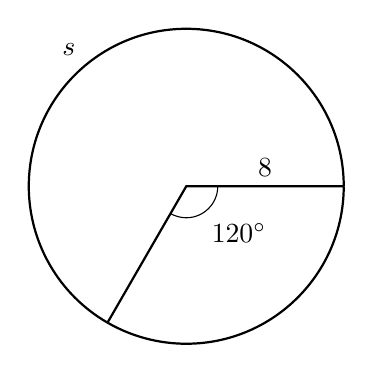
\begin{tikzpicture}[y=2cm, x=2cm,font=\sffamily]
  \draw[thick,black] (0:1) arc (0:240:1);
  \draw[thick,black] (0:1) -- (0,0) -- (240:1);
  \draw[thick,black] (0:1) arc (0:-120:1);

  \draw[black] (0.2,0) arc (0:-120:0.2);
  \node[anchor=south east] at (130:1) {$s$};
  \node[anchor=north west] at (300:0.2) {$120^\circ$};
  \node[anchor=south] at (0.5,0) {$8$};
\end{tikzpicture}


\end{enumerate}

